\documentclass[11pt]{article}\usepackage[]{graphicx}\usepackage[]{color}
% maxwidth is the original width if it is less than linewidth
% otherwise use linewidth (to make sure the graphics do not exceed the margin)
\makeatletter
\def\maxwidth{ %
  \ifdim\Gin@nat@width>\linewidth
    \linewidth
  \else
    \Gin@nat@width
  \fi
}
\makeatother

\definecolor{fgcolor}{rgb}{0.345, 0.345, 0.345}
\newcommand{\hlnum}[1]{\textcolor[rgb]{0.686,0.059,0.569}{#1}}%
\newcommand{\hlstr}[1]{\textcolor[rgb]{0.192,0.494,0.8}{#1}}%
\newcommand{\hlcom}[1]{\textcolor[rgb]{0.678,0.584,0.686}{\textit{#1}}}%
\newcommand{\hlopt}[1]{\textcolor[rgb]{0,0,0}{#1}}%
\newcommand{\hlstd}[1]{\textcolor[rgb]{0.345,0.345,0.345}{#1}}%
\newcommand{\hlkwa}[1]{\textcolor[rgb]{0.161,0.373,0.58}{\textbf{#1}}}%
\newcommand{\hlkwb}[1]{\textcolor[rgb]{0.69,0.353,0.396}{#1}}%
\newcommand{\hlkwc}[1]{\textcolor[rgb]{0.333,0.667,0.333}{#1}}%
\newcommand{\hlkwd}[1]{\textcolor[rgb]{0.737,0.353,0.396}{\textbf{#1}}}%
\let\hlipl\hlkwb

\usepackage{framed}
\makeatletter
\newenvironment{kframe}{%
 \def\at@end@of@kframe{}%
 \ifinner\ifhmode%
  \def\at@end@of@kframe{\end{minipage}}%
  \begin{minipage}{\columnwidth}%
 \fi\fi%
 \def\FrameCommand##1{\hskip\@totalleftmargin \hskip-\fboxsep
 \colorbox{shadecolor}{##1}\hskip-\fboxsep
     % There is no \\@totalrightmargin, so:
     \hskip-\linewidth \hskip-\@totalleftmargin \hskip\columnwidth}%
 \MakeFramed {\advance\hsize-\width
   \@totalleftmargin\z@ \linewidth\hsize
   \@setminipage}}%
 {\par\unskip\endMakeFramed%
 \at@end@of@kframe}
\makeatother

\definecolor{shadecolor}{rgb}{.97, .97, .97}
\definecolor{messagecolor}{rgb}{0, 0, 0}
\definecolor{warningcolor}{rgb}{1, 0, 1}
\definecolor{errorcolor}{rgb}{1, 0, 0}
\newenvironment{knitrout}{}{} % an empty environment to be redefined in TeX

\usepackage{alltt}
%Required: You must have these
\usepackage{graphicx}
\usepackage{tabularx}
\usepackage{natbib}
\usepackage{pdflscape}
\usepackage{array}
\usepackage{authblk}
\usepackage{gensymb}
\usepackage{amsmath}
%\usepackage[backend=bibtex]{biblatex}
\usepackage[small]{caption}

\setkeys{Gin}{width=0.8\textwidth}
\setlength{\captionmargin}{30pt}
\setlength{\abovecaptionskip}{10pt}
\setlength{\belowcaptionskip}{10pt}

 \topmargin -1.5cm 
 \oddsidemargin -0.04cm 
 \evensidemargin -0.04cm 
 \textwidth 16.59cm
 \textheight 21.94cm 
 \parskip 7.2pt 
\renewcommand{\baselinestretch}{1} 	
\parindent 0pt
\usepackage{setspace}
\usepackage{lineno}

\bibliographystyle{}
\usepackage{xr-hyper}
\usepackage{hyperref}


\title{Ranger Outline: We will come up with a better title when we feel more grounded in the results}
\date{}
\author{Dan, Cat, Nacho and Lizzie}
\IfFileExists{upquote.sty}{\usepackage{upquote}}{}
\begin{document}
\maketitle
\section*{Figures to make:}
\begin{enumerate}
\item Climate maps for species (some in supp. too)
\item Conceptual figure illustrating why variation in forcing should impact cue use
\item Results from cheapo models
\item some comparison of North America to Europe
\item Results from inter vs. intra specific model

\end{enumerate}
\section*{Abstract}
\section*{Introduction}
\textbf{For woody plants of the temperate zone the phenology, or annual timing, of spring budburst influences a myriad of ecological processes including patterns of resource allocation \citep{}, trophic interactions \citep{} and biogeochemical cycling \citep{}.}
 Through budburst timing, woody plants balance the advantages of precocious growth resumption for resource gains with the risk of damage from late season frost \citep{}. To navigate this tradeoff, woody plants have evolved complicated networks of sensory organs, hormone signaling, and physiological responses to sense environmental cues; changes in their physical environment, that signal the arrival of appropriate conditions for resuming growth.\\

\textbf{Decades of research suggest that warming spring temperatures (forcing), cool winter temperatures (chilling) and day length (photoperiod) are primary environmental cues utilized by woody plants that determine the timing of spring phenological events \cite{}}. These studies also demonstrate the there are substantial cue-use differences among species, with some species relying more heavily on some cues over others \citep{Laube:2014aa}. As anthropogenic climate change has already driven shifts in spring phenology \citep{}, identifying these interspecific differences in cue use has emerged as a major goal of phenological research \citep{}. These differences have strong implications for both predicting the rate of phenological shifts as the climate continues to warm \citep{}, and anticipating the ecological consequences of these shifts \citep{}.

\textbf{ But the quantification of cue use difference among species offers even more---a novel opportunity to interrogate long-standing theories regarding the biology underlying cue-use difference among species.} One particular relationship that can now be examined this the relationship species' geographic ranges and phenological cue use.

Climate is the major selective force on both species' geographic ranges \citep{} and their phenology \citep{}, and therefore, it is widely assumed that phenological cue-use differences among species reflect correlate with the climate of there repsecitve ranges \citep{}. That is, a species' relative reliance on forcing, chilling and photoperiod for each species should be shaped by the unique environmental conditions across a species' geographic range.\\

This has never really been tested (say better but see \citep{Zohner:2017aa}). With the recent quantification for cue use of many species \citep{} and the accessibility of high resolution climate data it is now possible to rigorously test this theory with data. Below, we briefly review the specific assumptions and predictions presented in the literature about the relationship between phenological cue-use and species' range characteristics. We then test these predictions using Bayesian models for a large suite of temperate woody species from North America and Europe.


\subsection*{Assumptions and predictions for the relationship between the cue-use and species' ranges}
\subsubsection{Relative reliance}
\begin{enumerate}
\item Assumptions:
\begin{enumerate}
\item Forcing is the predominant cure
\item Photoperiod and chill reliance evolves when forcing alone is not a reliable cue of safe growing condition \citep{Korner:2010aa}.
\item Forcing is an unreliable cue where there is significant variation in it.
\item Specific prediction species with high variation in forcing in there range should have a stronger response to chilling and or photoperiod and a weaker sensitivity to forcing. 
\item Yet, there are a few assumptions that need to be met in order to detect this signal if it is true.\\
\begin{enumerate}
\item Among species cue variation is higher than withing (ie cue use is ``conserved" at the species level)
\item There is coherance in forcing variation at multiple spatio-temporal scales.
\begin{enumerate}
\item Intra-annual variation (Temp.var ggdlf)
\item Inter-annual (cite Zohner) (Temp.var stv)
\item local cliamte variation (Geo.var ggdlf)
\item Deeper time stability \citep{} (literature)
\item global climate varaition (continents)

\end{enumerate}
\item Any of these level of varation could itself drive selecion for secondary cue usage (photoperiod/chilling) and it is unclear which is most important \citep{Zagmajster:2014aa}. If variation across these scales is not coherant clouding the signal.
\end{enumerate}
\item It may be also possible to test these hypotheses more indrectly through a range proxy.
\item Rappenports Rule suggests that increased cliamted isntability correlates with larger range spcies. This has been show for Temperature trees in North America\citep{Morin:2011aa}. If this is the case, species with larger ranges should have stronger chill/photoperiod cues
\end{enumerate}
\end{enumerate}
%\item Predictions from the literature
%\begin{enumerate}
%\item  Rappenports Rule \citep{Morin:2011aa} Species with larger ranges should have stronger chill/photoperiod cues
%\begin{eunumerate}
%\item  Assumption: Larger ranges have more variability \citep{Morueta-Holme:2013aa}
%end{enumerate}


\item We tested these underlying assumptions aboutt he relationship between cliamte variables in a species ranges and specific predictions for the relationship between range cliamte and cue use using the OSPREE database, and climate data, and models. % is this redunant. Could go in to more detail here.
\item Our interrogation of these relationships between climate and cue use not only clarifies the evolutionary drivers of cue use, but offers new insights regarding implications of climate change as both species' ranges and phenology continue to shift with warming.
\end{enumerate}
\section*{Methods}
\subsection*{Phenological data and cue-use estimates}
Dan and/or Lizzie write:
\begin{itemize}
\item Introduce OSPREE
\item Species selection
\item Model description
\end{itemize}

\subsection*{Species' range characteristics}
Cat and/or Nacho write?\\
\begin{itemize}
\item Climate data \textbf{(Figure of range maps with one climate variable, other could go to supplement)}
\item note on temp vs. geographic variation
\item calculation of GDD last frost
\item STV
\item range area
\end{itemize}


\subsection*{Statistical analysis}
\subsubsection*{Variation and secondary cue use}
Dan write description of cheapo models. Name them something cool. 
\subsubsection*{Intra vs. interspecific models}
Cat or Lizzie or Dan write

\section*{Results}
\subsection*{Intra vs. interspecific}
We found that inter-specific variation in cue us was higher than intraspecific.

\subsection*{Coherance of forcing variation}
Like Fig \ref{fig:climcor} but with:
\begin{itemize}
\item gddlf.temp by ggdlf.geo
\item stv by ggdlf.geo
\item stv by ggdlf.temp
\item area x ggdlf.temp
\end{itemize}

\subsection*{Climate variation and secondary cue use}

\subsection*{Climate variation, cues and Rappenport rule}

\section*{Discussion}


\begin{figure}[h!]
    \centering
 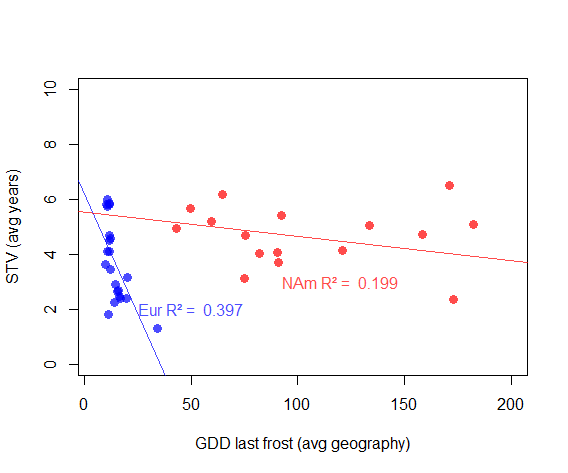
\includegraphics[width=\textwidth]{..//figures/STVvsGDDNamEu.png} 
    \caption{Correlations between levels of forcing variation. instead of this we'll SD_gglf.temp X SD_gglf.geo, STV X SD_gglf.geo, stv by SD_gglf.temp, and maybe area by some of these things too.}
    \label{fig:climcor}
\end{figure}


\end{document}
